\chapter{Tecnologías}
 En este capítulo se detalla todo lo relativo a los lenguajes de programación, los entornos de desarrollo y los \textit{frameworks} elegidos para llevar a cabo este proyecto, así como sus características principales y la razón de su uso.
    
    \section{Lenguajes de programación}
    
    \subsection{TypeScript}
    TypeScript\cite{typescript} es un lenguaje de programación orientado a objetos (OO) el cual es un superconjunto de JavaScript. Decimos que una tecnología es un superconjunto de un lenguaje de programación, cuando puede ejecutar programas de la tecnología . En resumen, ejecutará el código como si fuese JavaScript. \newline
        
    TypeScript se diferencia de JavaScript principalmente en que posee inferencia de tipos, es decir, está fuertemente tipado, además de algunas funcionalidades extra.
    \newline
        
    Este lenguaje se utiliza en el \textit{frontend} del proyecto, dado que el \textit{framework} elegido para realizar esta parte es Angular, el cual se explicará en detalle más adelante.
        
    \subsection{HTML-5}
    HTML-5\cite{html} (HyperText Markup Language) es la quinta revisión importante del lenguaje básico de la World Wide Web. Se trata de un lenguaje de marcación para la elaboración del contenido de las páginas web.
    Hoy en día es el lenguaje estándar que aceptan la gran mayoría de los navegadores a la hora de la construcción de las páginas web.
    \newline
     
    HTML-5 se diferencia de sus versiones anteriores en que incorpora nuevas etiquetas (section, article, header, footer etc...) con las cuales se busca mejorar y estandarizar la estructura de las páginas web además de otras actualizaciones como la mejora de los formularios o la inclusión de elementos de audio y vídeo.
    \newline
    
    Se ha optado por utilizar este lenguaje de marcación debido a su popularidad y a la inclusión de nuevas etiquetas que favorecen la lectura de la página web por parte de los navegadores.
    \newline
    
    \subsection{CSS-3}
    CSS\cite{css} (Cascading Style Sheets) es un lenguaje de diseño gráfico para definir y crear la presentación de un documento estructurado escrito en un lenguaje de marcado. Se utiliza en la mayoría de sitios web junto con HTML para generación de páginas web. De esta manera es mucho más sencillo generar páginas web, ya que, el diseño (CSS) se encuentra separado del contenido (HTML). \newline

    \subsection{Java 8}
    Java\cite{java} es un lenguaje de programación y una plataforma informática comercializada por primera vez en 1995 por Sun Microsystems\cite{sun} . Proviene de los lenguajes C y C++, y sus aplicaciones pueden ser ejecutadas en cualquier JVM (Java Virtual Machine).
    \newline
    
    Para este proyecto se ha utilizado la version 8 porque esta versión es la que menos \textit{bugs} tiene y la que mejora más la eficacia en el desarrollo y la ejecución de programas Java\cite{java8}. Además de estas razones, escogimos Java por ser un lenguaje orientado a objetos ideal para desarrollar proyectos \textit{API-REST}.
    
    \subsection{SQL}
    SQL\cite{sql} es un lenguaje declarativo estándar internacional de comunicación dentro de las bases de datos que nos permite el acceso y manipulación de datos en una base de datos.
    \newline
    
    Se decidió utilizar este lenguaje debido a su uso en el SGDB (Sistema de Gestión de Base de Datos) que utilizamos en el proyecto, MySQL. Además de esto, SQL es ideal para trabajar con JPA (Java Persistence API) en el \textit{backend} del proyecto.
    
     \section{Entornos de desarrollo}
     
     \subsection{Visual Studio Code}
     Visual Studio Code\cite{vsc} es un editor de código fuente desarrollado por Microsoft para Windows, Linux y macOS. Incluye soporte para la depuración, control integrado de Git, resaltado de sintaxis, finalización inteligente de código, fragmentos y refactorización de código.
    \newline
    
    En este proyecto se ha utilizado este entorno de desarrollo para gestionar un proyecto Angular, ya que este editor posee gran versatilidad a la hora de instalar plugins y gestionar diferentes lenguajes de programación de manera simultánea.
    
     \subsection{MySQL Workbench}
     MySQL Workbench\cite{mysql} se trata de un programa para gestionar, diseñar y administrar bases de datos relacionales, utilizado en nuestro proyecto a la hora de manejar datos de manera local. \\
     \newline
     Se decidió utilizar debido a que se ha usado previamente en nuestros estudios de grado en diversas asignaturas de manera productiva, además de que posee una versión gratuita.
     
     \subsection{PhpMyAdmin}
     Al igual que MySQL Worbench, se trata de una herramienta de gestión de bases de datos MySQL, pero con la diferencia que el acceso a esta herramienta es vía web, alojándose en un servidor.\\
     \newline
     Esta herramienta la utiliza Hostinger\cite{hostinger},  proveedor de alojamiento web donde se ha decidido alojar el proyecto para desplegarlo en la web.
     
     \subsection{GitHub}
     GitHub\cite{github} es un sistema de gestión de proyectos y control de versiones de código que funciona con git, el cual hemos utilizado para trabajar en equipo. Hemos creado tres repositorios; un repositorio para el \textit{frontend} del proyecto, otro repositorio para el \textit{backend} del proyecto y otro para guardar la memoria escrita en \LaTeX . \\
     \newline
     Se decidió utilizar este sistema debido a la familiaridad que poseemos con el mismo, lo que se traduce en efectividad y productividad en el flujo de trabajo del equipo.

     \subsection{Bitbucket}
     Bitbucket\cite{bitbucket} es, al igual que GitHub, un sistema de gestión de proyectos y control de versiones. No se tenía planificado utilizar este sistema, pero un cambio en la política de GitHub por el cual se nos impedía gestionar nuestros repositorios de manera privada, nos obligó a buscar otras opciones con versiones gratuitas en las cuales guardar el proyecto y gestionar sus diferentes versiones.
     \newline
     
     Tras una búsqueda de sistemas similares, nos decantamos por utilizar Bitbucket debido a la posibilidad de crear repositorios privados gratuitos e ilimitados para equipos pequeños (menos de 5 personas).
     
     \subsection{Eclipse}
     Eclipse\cite{eclipse} es una plataforma de software compuesto por un conjunto de herramientas de programación de código abierto multiplataforma para desarrollar aplicaciones.
     \newline
     
     A lo largo de nuestro paso por los estudios de grado en Ingeniería del Software, hemos utilizado este programa para desarrollar código, razón por la cual lo hemos escogido para la realización de la parte \textit{backend} del proyecto.
     
     
     \subsection{Overleaf}
     Overleaf\cite{overleaf} es un gestor online de proyectos escritos en \LaTeX. Gracias a los cursos formativos impartidos por la Oficina de Software Libre\cite{ucmsoftwarelibre} realizado en años anteriores y a los recursos puestos a disposición de los alumnos\cite{recursoslatex} nos animamos a realizar la memoria con este editor online y en lenguaje de maquetación \LaTeX.
     
     
         \subsection{MobaXterm}
     MobaXterm\cite{mobaxterm} es una herramienta muy versátil, entre sus funciones destacan la emulación de terminales o la conexión a un cliente SSH.
     \newline 
     
     En este proyecto lo utilizamos con el objetivo de conectarse al servidor remoto proporcionado por Hostinger\cite{hostinger}, en el cual albergamos el despliegue de la parte \textit{backend} de nuestro proyecto.\newpage
     
     
     \section{Frameworks}
     
     \subsection{Java Spring}
     Spring\cite{javaspring} es un \textit{framework} del lenguaje de programacion Java el cual nos permite desarrollar aplicaciones de manera más rápida, eficaz y corta, saltándonos tareas repetitivas y ahorrándonos líneas de código.
     \newline
     
     Una de las características que define  Java Spring de otros \textit{frameworks} es la inversión de control, por la cual, es el \textit{framework} y no el programador el que ejecuta ciertas operaciones sobre la aplicación, invirtiendo de esta manera los métodos de programación tradicionales.
     Otra de las características propias de Java Spring es la inyección de dependencias, por la cual Spring es capaz de crear o instanciar aquellos objetos que el programador necesite, favoreciendo el desacoplamiento y la manejabilidad de los mismos.
     Además de esto da soporte a una gran cantidad de \textit{frameworks} a través de dependencias, facilitando la tarea del programador.
     \newline
     
     Hemos escogido este \textit{framework} para realizar la parte \textit{backend} de nuestra aplicación por las características citadas anteriormente, construyendo una \textit{API-REST}. Esta \textit{API-REST} actúa como un servidor, siendo consumida por un cliente.
     \newline
    
    Spring da soporte a una gran cantidad de herramientas a través de dependencias. Dichas dependencias se gestionan mediante Maven\cite{maven}, una herramienta que simplifica los procesos de instalación.
    
    \begin{figure}[h]
    \centering
    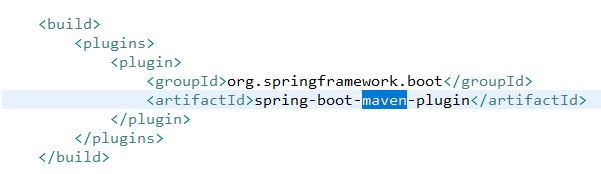
\includegraphics[width=1\textwidth]{images/maven}
    \caption{Instalación Maven en Java Spring}
    \end{figure}
    
    

        \subsubsection{\underline{Swagger}}
        Swagger\cite{swagger} es un proyecto \textit{open source} para describir, producir, consumir y visualizar aplicaciones \textit{API REST.} Para este proyecto vamos a utilizarlo con código Java, con el objetivo de generar la documentación de los puntos de acceso y de las entidades que se envían y se reciben.

        
        \subsubsection{\underline{Mockito}}
        Mockito\cite{mockito} es un \textit{framework} utilizado junto con JUnit\cite{junit} en Java para realizar tests de manera sencilla. En este proyecto se va a utilizar para testear las capas de \emph{Business} y \emph{Controller}, con el objetivo final de conseguir un 100\% de cobertura en las clases testeadas.
        \newline
        

        \subsubsection{\underline{JPA}}
        JPA\cite{jpa} (Java Persistence API) es una especificación de java para acceder, persistir y manejar datos entre Clases-Objetos de Java y bases de datos relacionales.
        \newline
        
        Gracias a los conocimientos de JPA adquiridos y desarrollados en las asignaturas de IS (Ingeniería del Software) y MS (Modelado de Software), nos decantamos por esta opción para gestionar las llamadas a las bases de datos correspondientes.
        

     \subsection{Angular}
       Angular\cite{angular} es un \textit{framework} de desarrollo de aplicaciones SPA (Single Page Applications), el cual utiliza Typescript como lenguaje de programación. Este \textit{framework} tiene la ventaja de que no refresca el navegador al modificar los elementos de la página web, dando una sensación de dinamismo y de inmersión al usuario.
       \newline
       
       Nos decantamos por utilizar este \textit{framework} debido a su popularidad y al gran uso que se le da a nivel empresarial.

        \subsubsection{\underline{Bootstrap}}
         Bootstrap\cite{bootstrap} es una herramienta para crear interfaces de usuario limpias y totalmente adaptables a todo tipo de dispositivos y pantallas, sea cual sea su tamaño.
         \newline
         
         Escogimos esta herramienta ya que nos proporciona resultados óptimos y limpios de manera rápida, además de que posee una extensa documentación\cite{documentationboostrap} a la que acudir en caso de duda.

   
     